\documentclass[aspectratio=169]{beamer}
\usetheme{Bruno}
\setbeamertemplate{footline}[frame number]
\usepackage{comment}
\usepackage{graphicx}

\title[IoT for Rural Aqueducts using MBSE]{Towards a Modular IoT System Architecture for Rural Aqueducts using Model-Based Systems Engineering}
\author[Tecnológico de Costa Rica]{Anthony José Arguedas-Rodríguez \and María José Angulo-Campos \and Juan José Montero-Jiménez \and Juan José Rojas-Hernández}
\date{2025 IEEE International Symposium on Systems Engineering}

\begin{document}

\begin{frame}
    \begin{center}
        {\LARGE \textbf{\inserttitle}} \\
        \vspace{0.5cm}
        {\insertauthor} \\
        \vspace{0.25cm}
        \includegraphics[height=2.3cm]{images/logo_delta.png} \raisebox{0.4cm}{\includegraphics[height=1.3cm]{images/logo_tec.jpg}} \raisebox{0.4cm}{\includegraphics[height=1.6cm]{images/logo_isse.png}} \\
    \end{center}
\end{frame}

\begin{frame}
    \frametitle{Contents}
    \begin{itemize}
        \item IoT Systems in Rural Aqueducts Context
        \item ARCADIA Model-Based Systems Engineering (MBSE) Methodology
        \item Operational Need Analysis: What Rural Aqueducts Need to Accomplish
        \item System Need Analysis: What IoT Systems Must Accomplish for Rural Aqueducts
        \item Logical Architecture: A Generic and Modular IoT System
        \item Physical Architecture: A Case Study of ASADA Paso Ancho, Costa Rica
        \item Conclusions and Future Work
    \end{itemize}
\end{frame}

\begin{frame}
    \frametitle{What are Rural Aqueducts?}

    \begin{columns}[T] % Align columns at the top
        \begin{column}{0.5\textwidth}
            \begin{enumerate}
                \item Self-managed
                \item Rural community-based
                \item Small-scale
                \item Limited staff
                \item Commonly resource-constrained
                \item Manual monitoring, inspection, and control methods
                \item Vulnerable to water loss and unreliable service
            \end{enumerate}
        \end{column}
        \begin{column}{0.5\textwidth}
            \begin{figure}
                \includegraphics[width=0.8\columnwidth]{images/asada.png}
                \caption{Aerial view of the water tank facility of ASADA Paso Ancho, Costa Rica.}
            \end{figure}
        \end{column}
    \end{columns}
\end{frame}

\begin{frame}
    \frametitle{\small IoT Systems in Rural Aqueducts Context}
    \framesubtitle{Previous Work on IoT Technology Transfer to Rural Aqueducts at Laboratorio Delta}

    \begin{columns}[T] % Align columns at the top
        \begin{column}{0.5\textwidth}
            \begin{figure}
                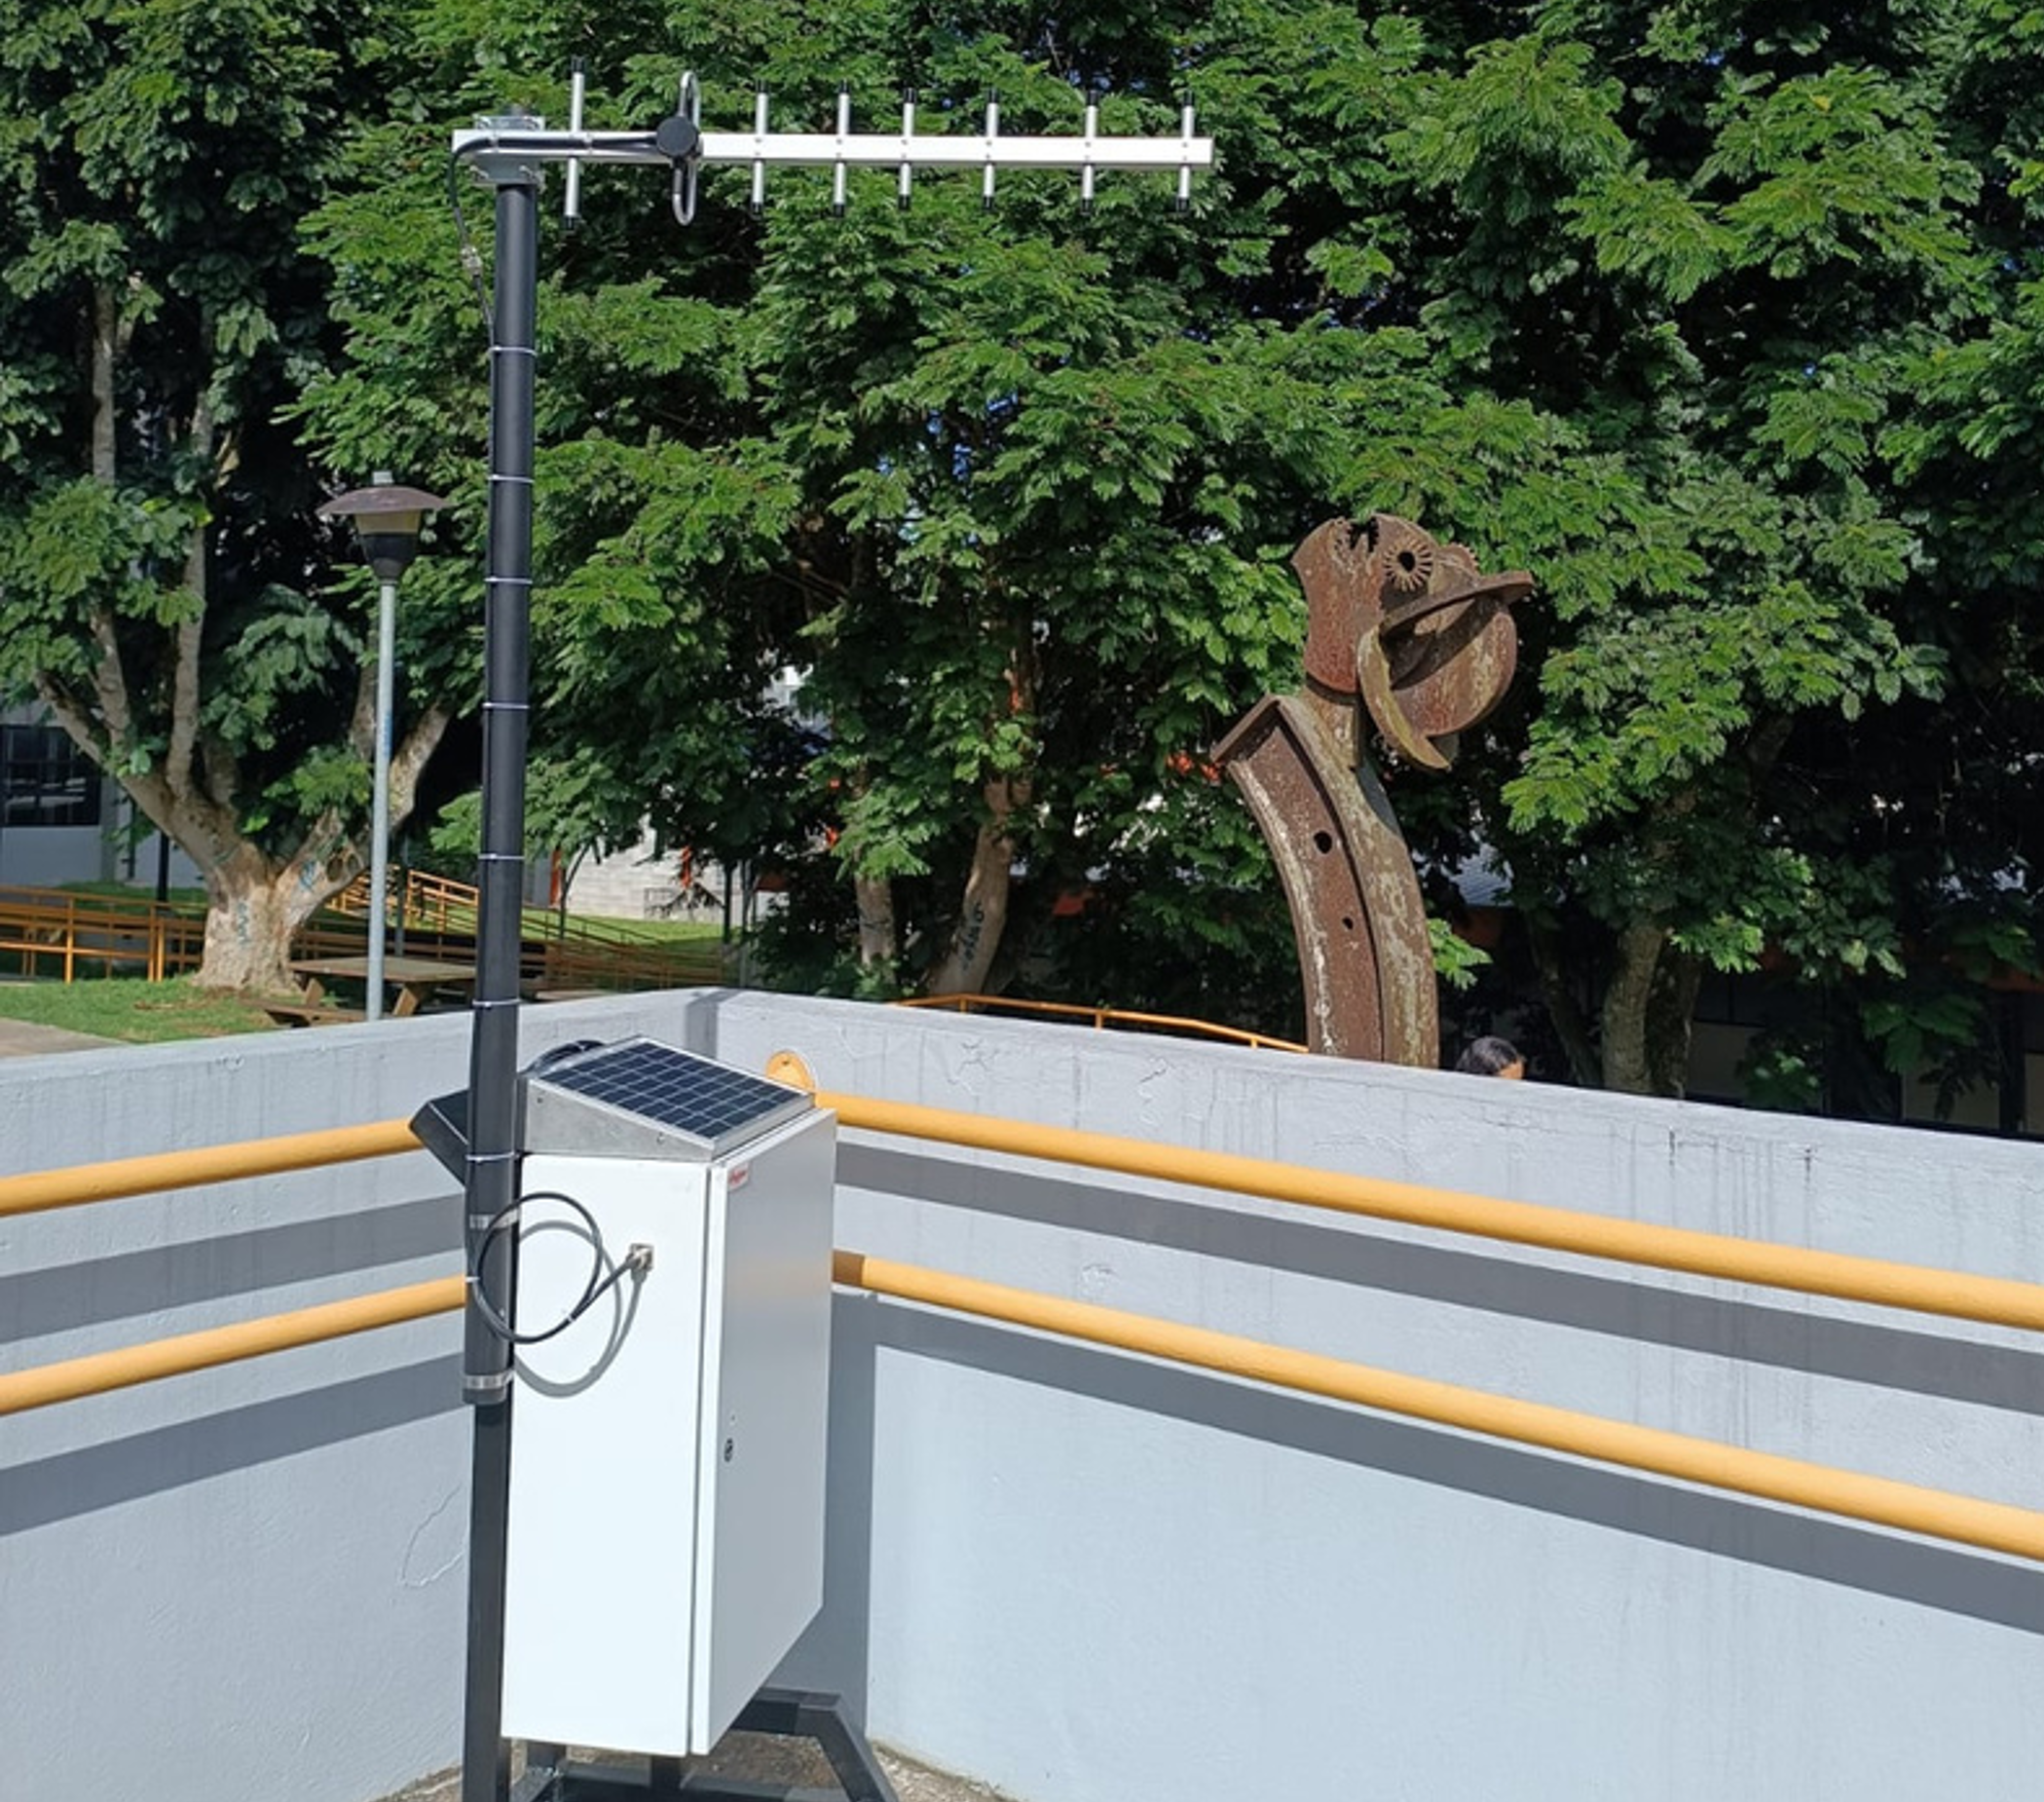
\includegraphics[width=0.7\columnwidth]{images/oviedo.png}
                \caption{IoT system developed by [1] for ASADA Paso Ancho, Cartago.}
            \end{figure}
        \end{column}
        \begin{column}{0.5\textwidth}
            \begin{figure}
                \includegraphics[width=0.8\columnwidth]{images/solorzano.png}
                \caption{IoT system developed by [2] for ASADA Playa Sámara, Nicoya.}
            \end{figure}
        \end{column}
    \end{columns}
\end{frame}

\begin{frame}
    \frametitle{Research Questions}

    \begin{itemize}
        \item \textbf{RQ1:} Are there existing systems engineering-based (including ARCADIA MBSE) architectures for the design of IoT systems for rural aqueducts?
        \item \textbf{RQ2:} If they exist, are the architectures generic and modular?
        \item \textbf{RQ3:} What are the needs and desires of rural aqueducts that can be addressed by IoT systems?
        \item \textbf{Contribution:} A generic system architecture for rural aqueducts, developed using the ARCADIA method
    \end{itemize} 
\end{frame}

\begin{frame}
    \frametitle{The ARCADIA MBSE Methodology}

    \begin{figure}
        \centering
        \includegraphics[width=0.9\textwidth]{images/phases_arcadia.png}
        \caption{Phases of the ARCADIA Model-Based Systems Engineering Methodology and its associated Language and Tool Capella.}
    \end{figure}
\end{frame}

\begin{frame}
    \frametitle{\small Operational Need Analysis}
    \framesubtitle{Extracting Generic Needs and Desires about IoT Systems in Rural Aqueducts using NLP}

    \begin{table}
        \centering
        \caption{Needs and desires extracted from paper full text embeddings using BERTopic.}
        \begin{tabular}{c p{6cm}}
            Code & Need or desire \\
            \hline
            ND1.1 & Identify sources of water pollution \\ %
            ND1.2 & Monitor water pollution \\ %
            ND2 & Monitor water pH \\ %
            ... & ... \\ %
            ND52 & MQTT node communication \\
            ND53 & Mobile network connectivity \\
            ND54 & WiFi connectivity \\
            ND55 & LoRaWAN connectivity \\
            \hline
        \end{tabular}
        \label{tab:clusters}
    \end{table}
\end{frame}

\begin{frame}
    \frametitle{\small Operational Need Analysis: Operational Capabilities}
    \framesubtitle{1: Provide high-quality water, 2: Comply with water quality standards and 4: Share data with external entities}

    \begin{figure}
        \centering
        
\includegraphics[width=\textwidth]{images/opcap1.jpg}
        \caption{Operational Need Analysis for rural aqueducts, reduced to the activities involved in Capabilities 1, 2 and 4.}
    \end{figure}
\end{frame}

\begin{frame}
    \frametitle{\small Operational Need Analysis}
    \framesubtitle{Operational Capability 3: Mitigate water loss}

    \begin{figure}
        \centering
        \includegraphics[width=0.9\textwidth]{images/opcap3.jpg}
        \caption{Operational Need Analysis for rural aqueducts, reduced to the activities involved in Capability 3.}
    \end{figure}
\end{frame}

\begin{frame}
    \frametitle{\small System Need Analysis: System Capabilities}
    \framesubtitle{1: Provide water quality data, 5: Share data with external entities}

    \begin{figure}
        \centering
        
\includegraphics[width=0.9\textwidth]{images/scap1-5.jpg}
        \caption{System Need Analysis for IoT systems in rural aqueducts, reduced to the activities involved in Capabilities 1 and 5.}
    \end{figure}
\end{frame}

\begin{frame}
    \frametitle{\small System Need Analysis: System Capabilities}
    \framesubtitle{2: Provide water loss data, 3: Provide water supply and demand data, 4: Control water distribution}

    \begin{figure}
        \centering
        
\includegraphics[width=0.85\textwidth]{images/scap2-3-4.jpg}
        \caption{System Need Analysis for IoT systems in rural aqueducts, reduced to the activities involved in Capabilities 2, 3 and 4.}
    \end{figure}
\end{frame}

\begin{frame}
    \frametitle{\small Logical Architecture Definition}
    \framesubtitle{Implementing modularity with end-user and environmental interactions}

    \begin{figure}
        \centering
        
\includegraphics[width=0.77\textwidth]{images/separation.jpg}
        \caption{Logical architecture for IoT systems in rural aqueducts, reduced to the logical componentes that interact with end-users and the environment.}
    \end{figure}
\end{frame}

\begin{frame}
    \frametitle{\small Logical Architecture Definition}
    \framesubtitle{Implementing modularity with buses, queues, and pub/sub channels}

    \begin{figure}
        \centering
        
\includegraphics[width=0.75\textwidth]{images/component_exchanges.jpg}
        \caption{Logical architecture for IoT systems in rural aqueducts, reduced to logical components and their component exchanges.}
    \end{figure}
\end{frame}

\begin{frame}
    \frametitle{\small Physical Architecture Definition}
    \framesubtitle{Implementing Logical Components}

    \begin{figure}
        \centering
        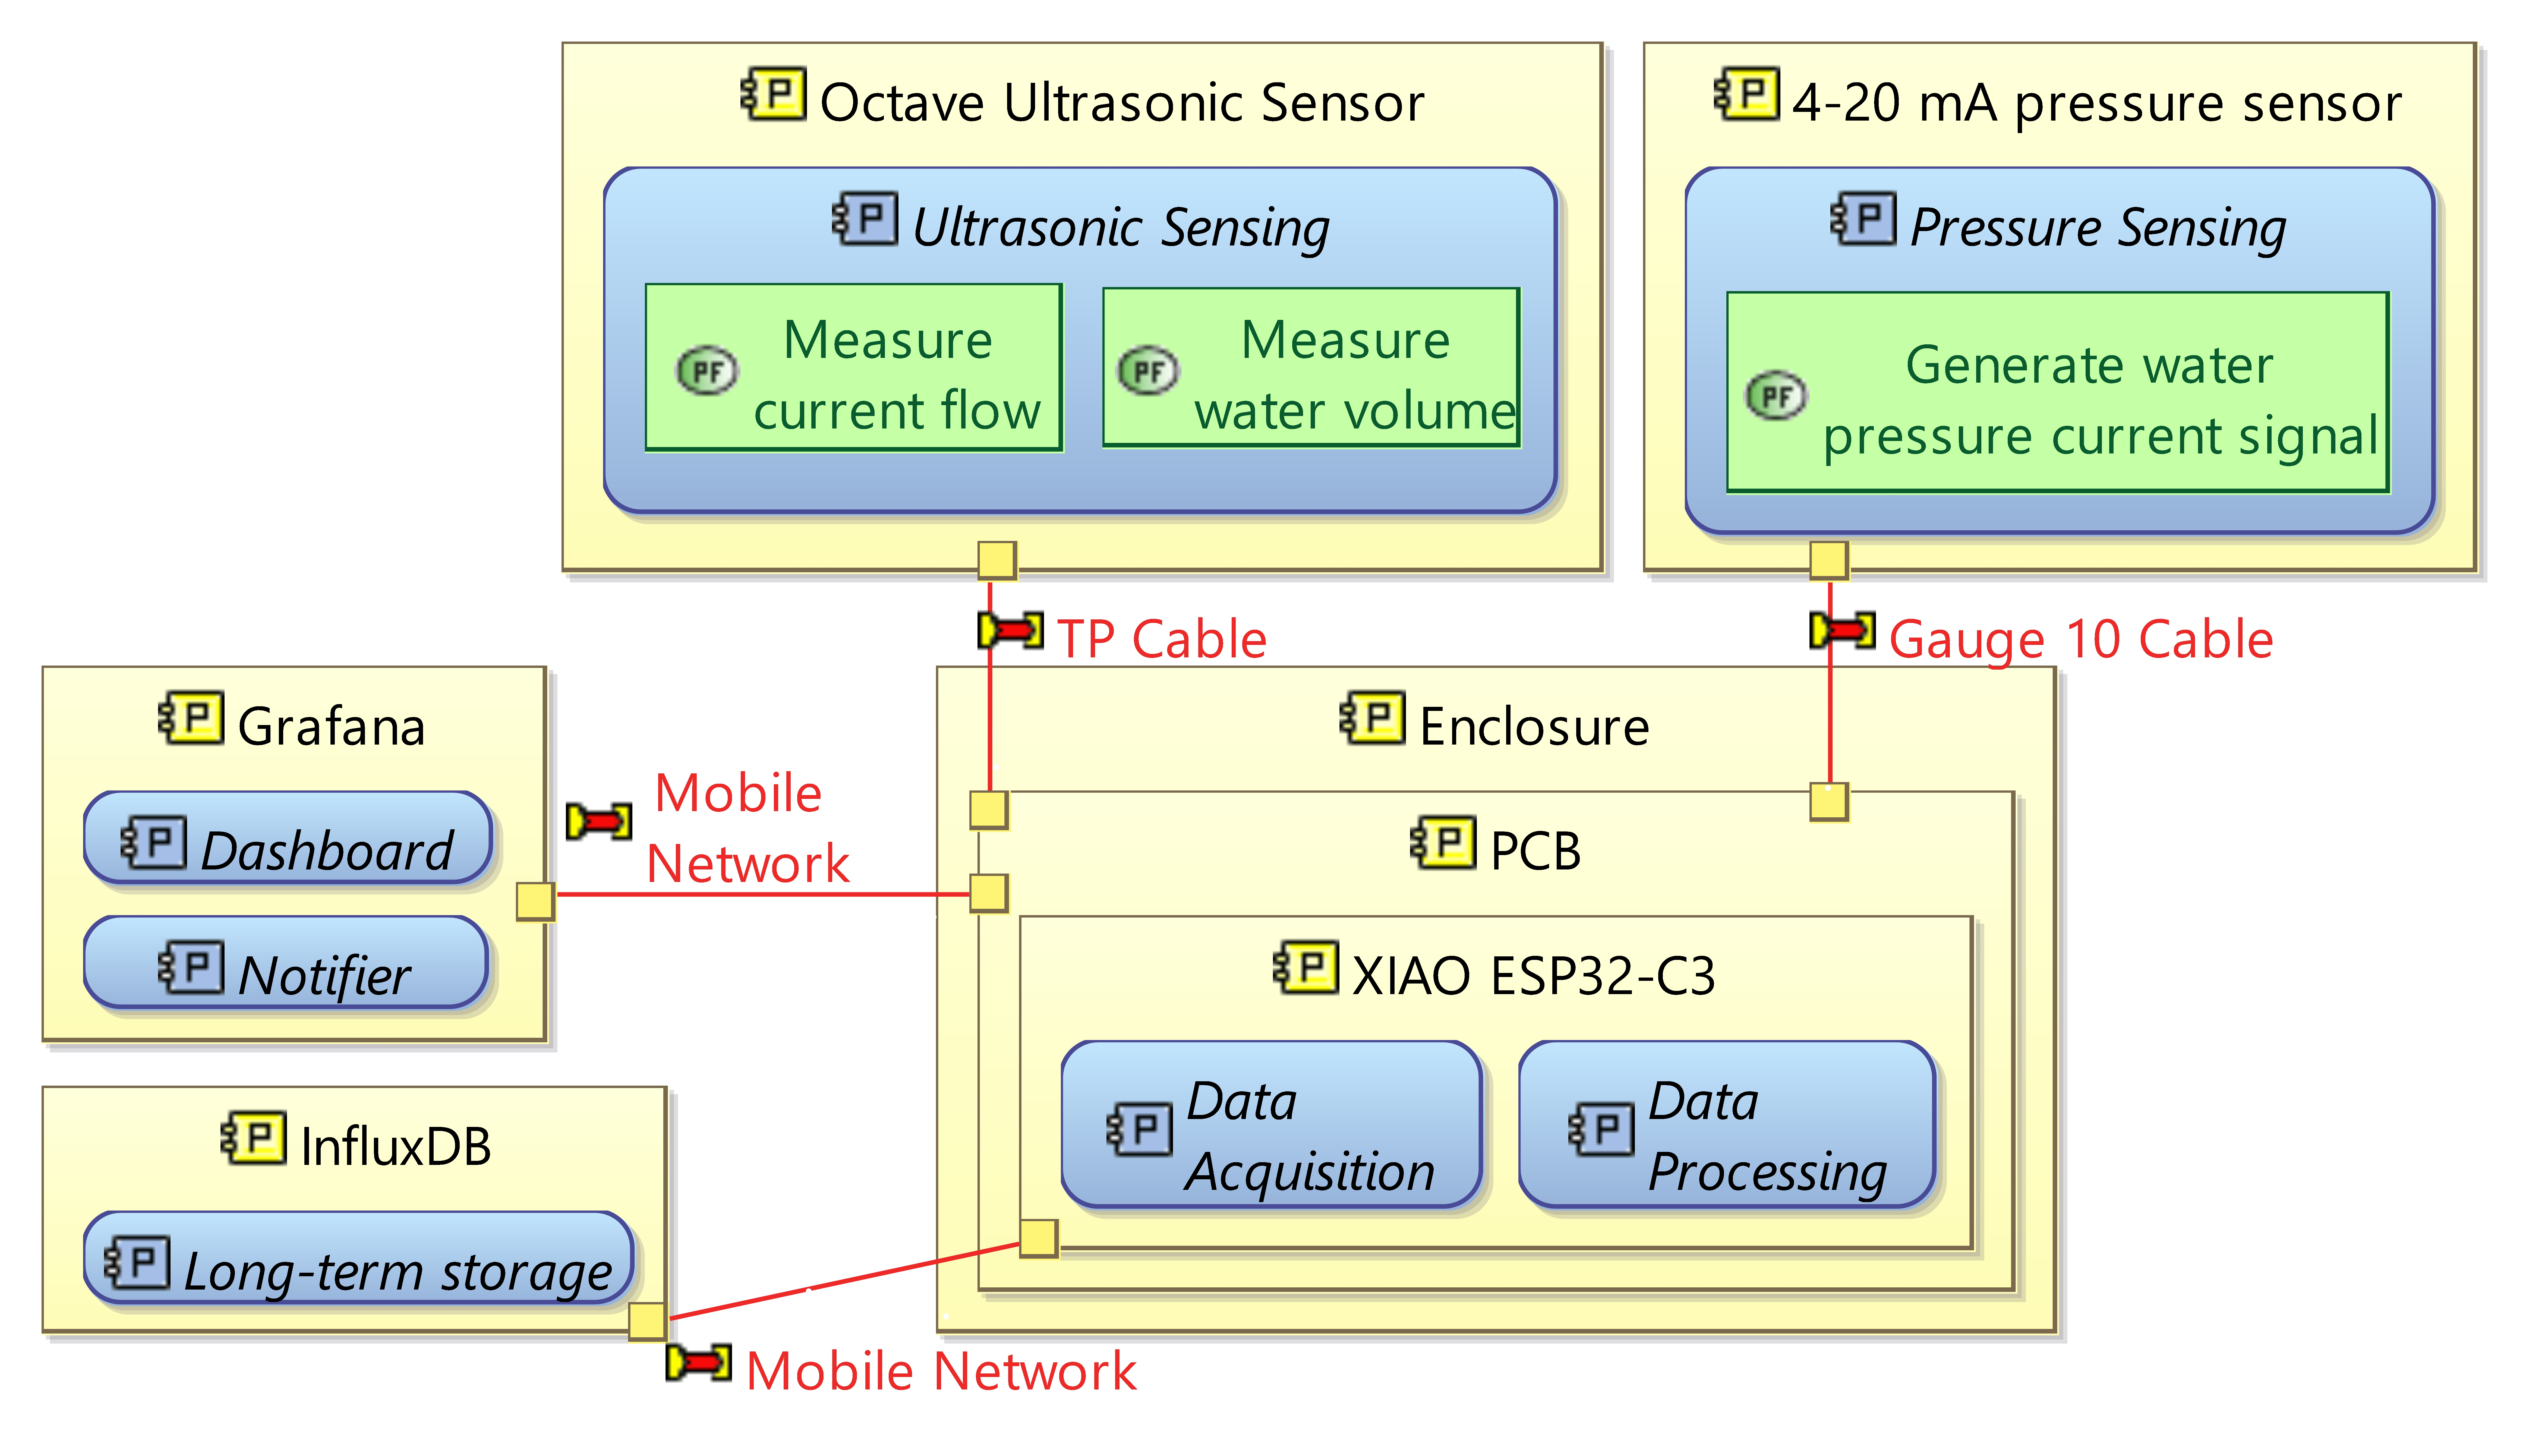
\includegraphics[width=0.65\textwidth]{images/physical_implementation.jpg}
        \caption{Physical architecture for IoT systems in rural aqueducts, reduced to the Physical Components implementing the Logical Architecture.}
    \end{figure}
\end{frame}

\begin{frame}
    \frametitle{\small Physical Architecture Definition}
    \framesubtitle{Introducing Implementation-Specific Functions}

    \begin{figure}
        \centering
        
\includegraphics[width=0.9\textwidth]{images/physical_new.jpg}
        \caption{Physical architecture for IoT systems in rural aqueducts, reduced to implementation-specific functions not found in the Logical Architecture.}
    \end{figure}
\end{frame}

\begin{frame}
    \frametitle{Conclusions and Future Work}

    \begin{itemize}
        \item Generality was introduced by extracting needs and desires from a wide range of literature using data mining techniques.
        \item The application of the ARCADIA MBSE method enabled traceability from needs to logical and even physical architecture, and technology-agnostic design.
        \item Modularity was achieved by separating end-user and environmental interactions, and by using buses, queues, and pub/sub channels for component exchanges.
        \item The presented architecture can be adapted to a practical implementation, for example by technology transfer initiatives.
        \item Future work should strengthen the data mining pipeline by including more sources of information, and further developing the physical architecture with more case studies.
    \end{itemize}
\end{frame}

\begin{frame}[allowframebreaks]
  \frametitle{References}
  \footnotesize
  \begin{thebibliography}{99}
    \bibitem{oviedo2024}
      A.~Oviedo Muñoz,
      ``Desarrollo de un prototipo para recopilación y monitoreo remoto de datos hídricos de los tanques, basado en dispositivos IoT, en la ASADA Paso Ancho y Boquerón,'' Specialization Practice Report to qualify for the title of Industrial Maintenance Engineer, Tecnológico de Costa Rica, Escuela de Ingeniería Electromecánica, Mar. 2024.
    \bibitem{solorzano2021}
      S.~Solórzano Alfaro,
      ``Sistema de control y monitoreo hídrico, basado en LoRaWAN, para el acueducto principal de la sociación administradora del acueducto rural de Playa Sámara de Nicoya,'' Specialization Practice Report to qualify for the title of Industrial Maintenance Engineer, Tecnológico de Costa Rica, Escuela de Ingeniería Electromecánica, Jun. 2021.
  \end{thebibliography}
\end{frame}

\begin{frame}
    \frametitle{\small Backup Slide}
    \framesubtitle{NLP Pipeline for Generic Needs and Desires Extraction}

    \begin{figure}
        \centering
        \includegraphics[width=\textwidth]{images/bertopic.png}
        \caption{Process of extracting generic needs and desires about IoT systems in rural aqueducts from published literature.}
    \end{figure}
\end{frame}

\end{document}
